\begin{figure}
\centering
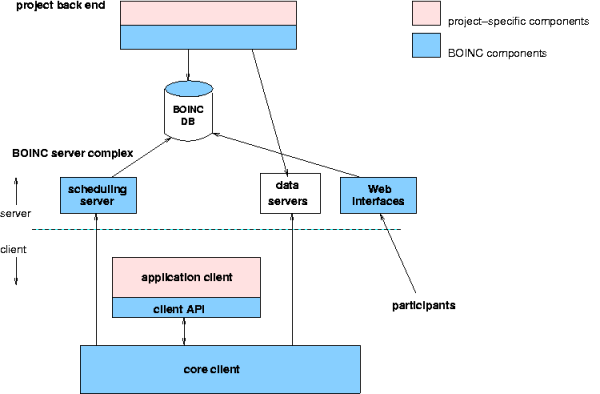
\includegraphics[scale=0.5]{figures/project_boinc}
\medskip
\caption{\textit{BOINC Client/Server Architecture} [5]}
\small
\end{figure}

\section{Rewarding Researchers}

Gridcoin does not only want to reward holders of the coin (as in pure Proof of Stake coins such as Peercoin [2]), but wants to reward researchers. Because of this there is an additional reward depending on the amount of research done. This information is read from a superblock. In some blocks, called superblocks, the majority consensus from the distributed Neural Network, which user has done how much work is also saved as a hash. These blocks are generated once a day. The current amount of research done by each CPID stored in the last superblock can be viewed on \texttt{www.gridcoinstats.eu}. If a node gets chosen and the hash this node contains about the amount of work done by this user is the same as the majority hash stored in the Neural Network, then this node gets to stake the next block and everything starts again. The actual reward the node gets then depends on the \textit{RAC} (Recent Average Credit [22]) for each project for this user as stored in the superblock.\\

\subsection{Cobblestone}

To understand \textit{RAC}, we first look at the \textit{cobblestone} [22]. The \textit{cobblestone} is a unit of measure defined as follows: it is 1/200 day (=7 minutes and 12 seconds or 432 seconds) of CPU time on a reference computer that does 1 Gigaflop (= 1 billion floating point operations per second) based on the Whetstone benchmark. A \textit{cobblestone} in other words correspond to 432 seconds * 1 Gigaflop = 432 billion floating point operations.\\


\subsection{Recent Average Credit (RAC)}

Cobblestones are converted into a certain number of "credits" on a project-by-project basis. The unit of conversion is not monitored by BOINC, and hence some projects grant more credits per cobblestone than others. However, this discrepancy does not affect Gridcoin payouts, since a researcher's output for a given project is normalized by the overall output of Gridcoin researchers \textit{within the same project} (see section 5.3).  

Besides tracking the \textit{total} computational output of a researcher (measured in total credits), BOINC also calculates a quantity called the Recent Average Credit (RAC), which is a time-averaged measure of computational \textit{power} (credits per unit time). More precisely, RAC is an exponentially weighted moving average over computational power, thus granting more weight to recently earned credits. The details of its calculation are as follows.

Generally speaking, an exponential moving average $S_i$ of a fixed-interval time series $X_i$ is a moving average which assigns exponentially less weight to data points in the past. More precisely,
\begin{equation}
S_i = (1-\alpha)^i X_0 + \alpha \sum_{j = 1}^i (1-\alpha)^{j-1} X_{i-j+1}
\end{equation} 
where $0 < \alpha < 1$ is a constant weighting factor. A large $\alpha$, corresponding to smaller $1-\alpha$, assigns smaller weight to data points in the past. $S_i$ can also be computed recursively for $i > 1$:
\begin{equation}
S_i = \alpha X_i + (1-\alpha) S_{i-1}.
\end{equation}
with $S_0 \equiv X_0$. This moving average can be understood intuitively using figure XXX. The output is $S_i$, and the input is $X_i$. As the input jumps to 1 the output slowly follows and wants to go to 1 as time passes. When the input changes this just repeats. The input’s rapid jump to 2 did not really make it to the output. Thus, $S_i$ has a smoothing effect on the relatively noisy series $X_i$ [31]. \\
We want to implement something similar for computational power. On the other hand, generally BOINC updates its statistics at uneven time intervals $\ldots <  t_{i-2} < t_{i-1} < t_i$, and hence a time-dependent weight $\alpha$ must be defined. BOINC has found it convenient to use the exponential weighting factor:
\begin{equation}
\alpha_i = 1 - \mathrm{e}^{-(t_i-t_{i-1}) \cdot  \ln(2) / th}  
\end{equation}
where $t$ is given in days. The BOINC source code works equivalently in terms of the weight function 
\begin{equation}
w(t_i - t_{i-1}) \equiv \mathrm{e}^{-(t_i-t_{i-1}) \cdot  \ln(2) / th}.
\end{equation}
 The quantity $th$ is called the halving parameter, since
\begin{equation}
w(t_i - t_{i-1})  =  \left( \mathrm{e}^{-\ln(2)} \right)^{(t_i-t_{i-1})/th} = \bigg(\frac{1}{2}\bigg)^{(t_i-t_{i-1})/th}
\end{equation}
using elementary properties of logarithms. BOINC has found it convenient to set $th$ equal to 7 days. Note that when $t_i - t_{i-1}$ is large, $\alpha_i$ is close to $1$, thus indeed granting exponentially less weight to older computations. In fact, if RAC is updated weekly, credit from 1 week ago is granted half the weight, credit from 2 weeks ago is granted one-quarter the weight, etc. Roughly speaking, credit from more than 2 months ago will not contribute significantly. \\
Let's put all of this together. Suppose the computational power at time $t_i$ is $R_i$. Having defined $RAC(t_i)$ in the above as the weighted moving average of the previous $R_i$, we have:
\begin{equation}
RAC(t_i) = \left[1 - w(t_i - t_{i-1})\right] R_i + w(t_i - t_{i-1}) \cdot RAC(t_{i-1}).
\end{equation}

\begin{figure}
\centering
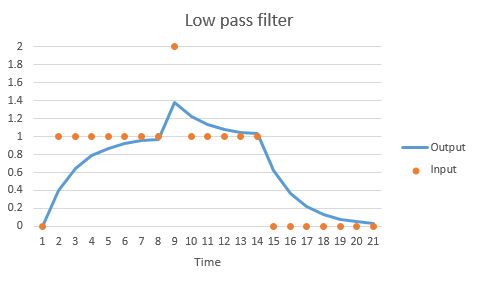
\includegraphics{figures/low-pass}
\caption{\textit{An exponential moving average in action smooths spikes and dips}}
\small
\end{figure}

\subsection{Gridcoin Payout to User Running Multiple Projects}

We hereby define:
\begin{description}
  \item{$\gamma$} : this is the \textit{RAC} done by a user on a particular BOINC project \textit{p} since last payment to user \textit{u} identified by \textit{CPID}.
  \item{$\Gamma$} : this is the \textit{RAC} done by all users participating in Gridcoin on a particular BOINC project \textit{p} since last payment to user \textit{u}.
  \item{$\tau$} : this is the time expressed in days since last payment to user \textit{u}.
  \item{$\Theta$} : this is the available Gridcoin supply per day assigned to BOINC project \textit{p}
  \item{$G$} : this is the constant number of Gridcoins created per day on the Gridcoin network. 
  \item{$n$} : this is the number of BOINC projects in the Whitelist [42]. Participants in whitelisted projects do receive a reward in Gridcoins for their computational effort.  
\end{description}

The ratio
\[\gamma/\Gamma\]
is the percentage of work done by user \textit{u} on BOINC project \textit{p} in respect to all other Gridcoin users working on project \textit{p}.\\

The amount of coins $\sigma$ for project \textit{p} the user \textit{u} gets, if he was only running project \textit{p}, is computed:
\[ \sigma = (\gamma / \Gamma) \cdot \tau \cdot \Theta \]

As of now the $\Theta$ is the same for each project, so
\[ \Theta = G/n \]

$\gamma$ and $\Gamma$ are calculated so that in case there were several superblocks since the last payment the average RAC of all those superblocks is used.\\

The $researchreward$ for user \textit{u} is then the sum of the rewards for each whitelisted project:

\[ researchreward = \sum_{p=1}^{n} \sigma(p) \]


The $totalreward$  for user \textit{u} is then the reward for the research done by this node plus the reward that any node gets for staking a block, called $inflationreward$ in the next formula:
\[ totalreward = inflationreward +  researchreward \]

The $inflationreward$ depends on the time that passed since the last stake is chosen in a way that it leads to an interest rate of 1.5\% per year.\\

The rewards that contain only $inflationreward$ and no $researchreward$
are often called PoS (Proof of Stake) rewards, whereas the rewards containing $inflationreward$ plus $researchreward$ are called Proof of Research rewards.
